\documentclass[a4paper]{article}

\usepackage[english]{babel}
\usepackage[utf8]{inputenc}
\usepackage{fullpage}
\usepackage{amsmath}
\usepackage{graphicx}
\usepackage[colorinlistoftodos]{todonotes}
%\usepackage{hyperref}
\usepackage{amssymb}
\usepackage{subfigure}
\usepackage{url}
\usepackage[pagebackref=true,colorlinks,linkcolor=red,citecolor=green,breaklinks=true,bookmarks=false]{hyperref}
\usepackage{outline} 
\usepackage{pmgraph} \usepackage[normalem]{ulem}
\usepackage{graphicx} \usepackage{verbatim}
\usepackage{indentfirst}
\usepackage{listings}
\usepackage{xcolor}
\lstset{
	numbers=left, 
	numberstyle= \tiny, 
	keywordstyle= \color{ blue!70},
	commentstyle= \color{red!50!green!50!blue!50}, 
	frame=shadowbox, % 阴影效果
	rulesepcolor= \color{ red!20!green!20!blue!20} ,
	escapeinside=``, % 英文分号中可写入中文
	xleftmargin=2em,xrightmargin=2em, aboveskip=1em,
	framexleftmargin=2em
} 
\setlength{\parindent}{2em}
% \usepackage{minted} % need `-shell-escape' argument for local compile

\title{
	\vspace*{1in}
	
\includegraphics[width=2.75in]{figures/zhenglab-logo} \\
	\vspace*{1.2in}
	\textbf{\huge Weekly Work Report}
	\vspace{0.2in}
}

\author{Hongzhi Liu \\
	\vspace*{0.5in} \\
	\textbf{VISION@OUC} \\
	\vspace*{1in}
}

\date{\today}


\begin{document}
	\par
	\maketitle
	\setcounter{page}{0}
	\thispagestyle{empty}
	
	\newpage
	
	\section{Research problem}
	
	During this week's short and tense preparation time, our team take much efforts to deal with hardware and software problems. First, we need to counterweight for open ROV equipment in order to smooth the equipment in the water. Then we should try to make the Faster RCNN algorithm read the video stream from the device normally, object recognition and number counting when equipment is in the water. Besides, I prepare and test some model weights for contest that can help us to choose a better one with high mAP. Furthermore, I train two online model weights to detect holothurian, echinus, scallop and number one to six which representative six regions. 
	
	Because of difficulty in code modification for online algorithm version, I have little time for improving online recognition accuracy and performance. Until the day before the competition, we are still adjusting and modifying the algorithm codes in order to keep device in a better state and be able to get a ideal result. Fortunately, we run smoothly on the day of code running and the operation equipment as well.	
		
	\section{Research approach}
	
	In the process of contest preparation, I use the method of documentary analysis, comparative analysis and experimental research method. I read the thesis of RCNN\cite{Girshick2014}, Fast R-CNN \cite{Girshick2015Fast} and Faster R-CNN algorithm \cite{Ren2015Faster}. I try to unferstand core ideology in paper and learn about concept introduced by author.
	
	Besides, I learn grammatical application of python on the one hand, and on the other hand, I try to write code files to achieve the goal. By this method, I can have a better understanding of python.
	
	For deep learning, I watch the fifth course videos and write down the issues which I think are much important for further research. And then, I not only have learned the lessons of deep learning, but also put them into coding action. 
	
	
	\section{Research progress}
	
	During preparation for URPC2018, I have trained offline and online models for competition and evaluate how good the restoration algorithm are with mAP values. I continue to test origin pictures about Faster R-CNN algorithm \cite{Ren2015Faster}. Besides, I change different threshold value to test picture in order to get a better mAP. And I will list details about weekly work in Tab.~\ref{t1} below.

	
	\begin{table}[hb]
		\centering
		\caption{Weekly work progress.}
		\begin{tabular}{c|p{10cm}}
			\hline 
			& Finish training offline and online models for competition.\\
			
			URPC2018& Finish comparing results of different threshold. \\
			
			& Finish comparing mAP value of different methods and judge which are better.\\
			
			& Finish online and offline tests on site.\\

			\hline
			Deep Learning& Finish learning Sequence Models which is the fifth course of deep learning.\\
			\hline
		\end{tabular}
		\label{t1}
	\end{table} 
	
		
		\begin{figure}
			\begin{center}
				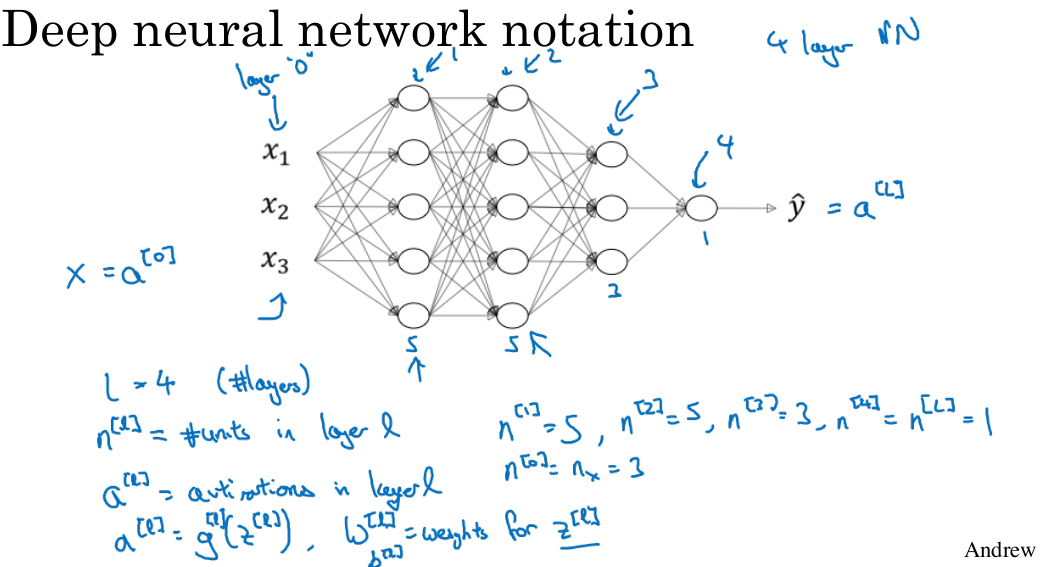
\includegraphics[scale=0.6]{figures/1.png}
			\end{center}
			\caption{Output test results of several models.}
			\label{p1}
		\end{figure}
	
	\begin{figure}
		\centering 
		\subfigure[]{ 
			\label{p2a} %% label for first subfigure 
			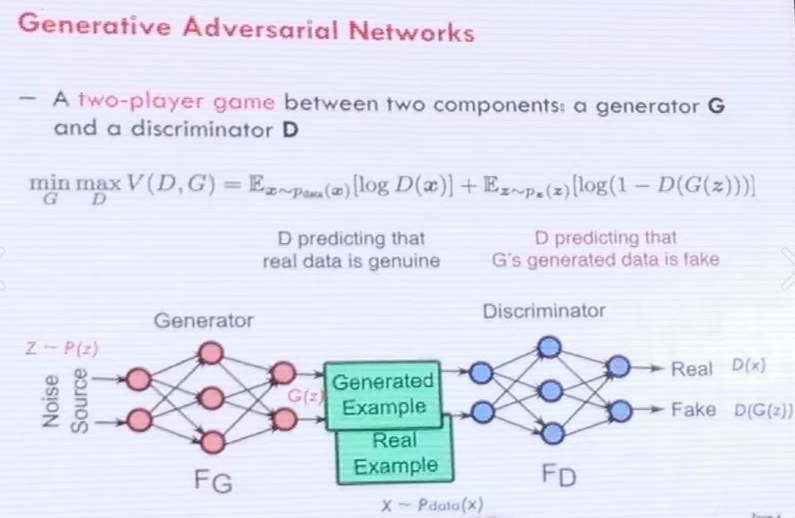
\includegraphics[width=7cm]{figures/2.png} 
		} 
		\subfigure[]{ 
			\label{p2b} %% label for second subfigure 
			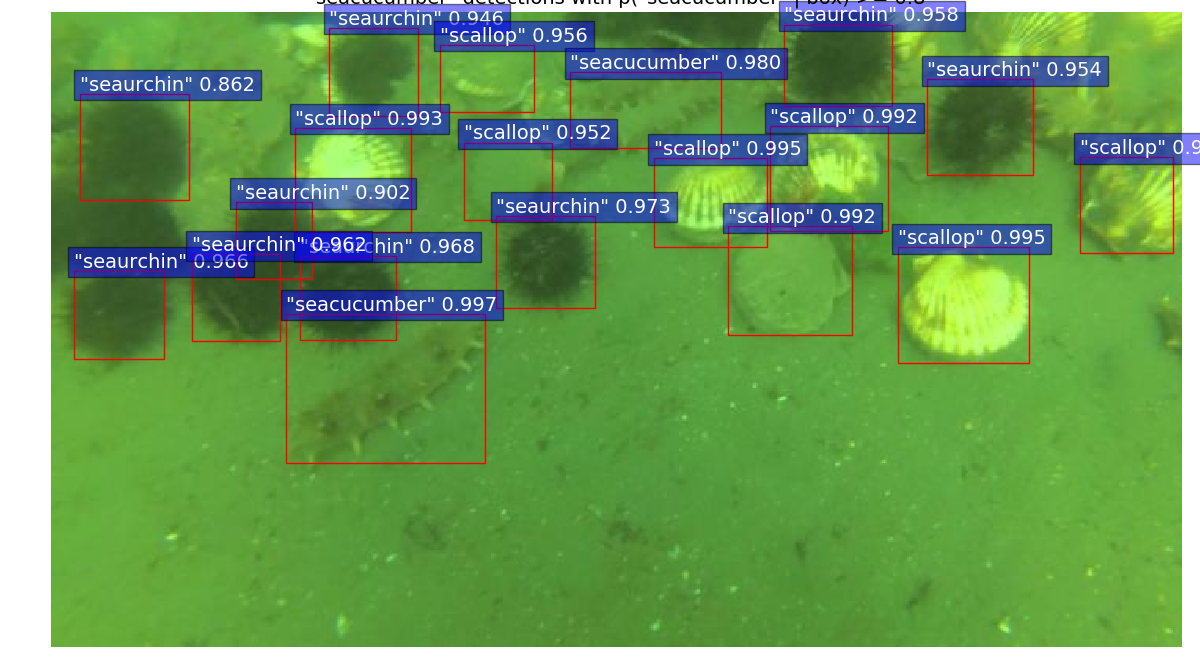
\includegraphics[width=7cm]{figures/3.png} 
		} 
		\subfigure[]{ 
			\label{p2c} %% label for second subfigure 
			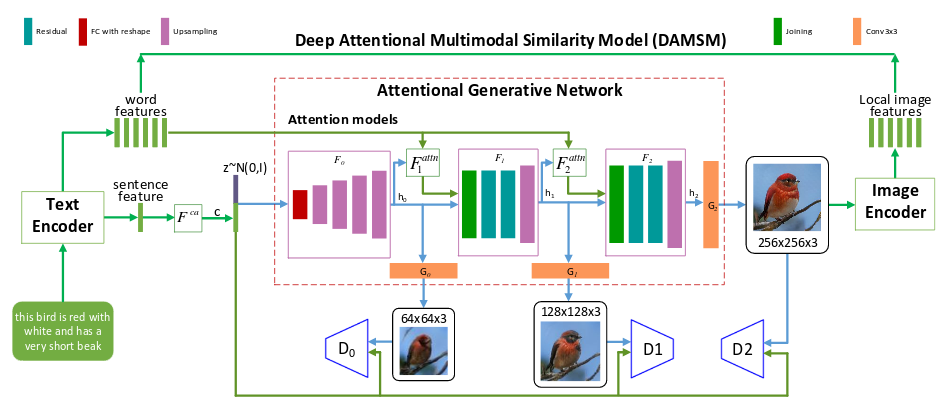
\includegraphics[width=7cm]{figures/4.png} 
		}
		\subfigure[]{ 
			\label{p2d} %% label for second subfigure 
			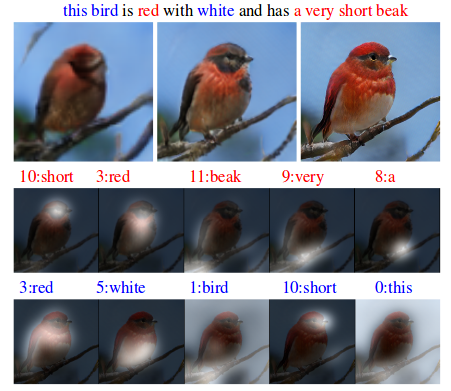
\includegraphics[width=7cm]{figures/5.png} 
		}
		\caption{Contest result of different models that are origin model (or yuantu model), enhanced model, 17\&18 model and dcp model.} 
		\label{p2} %% label for entire figure 
	\end{figure}  
	
	\begin{figure}
		\centering 
		\subfigure[]{ 
			\label{p3a} %% label for first subfigure 
			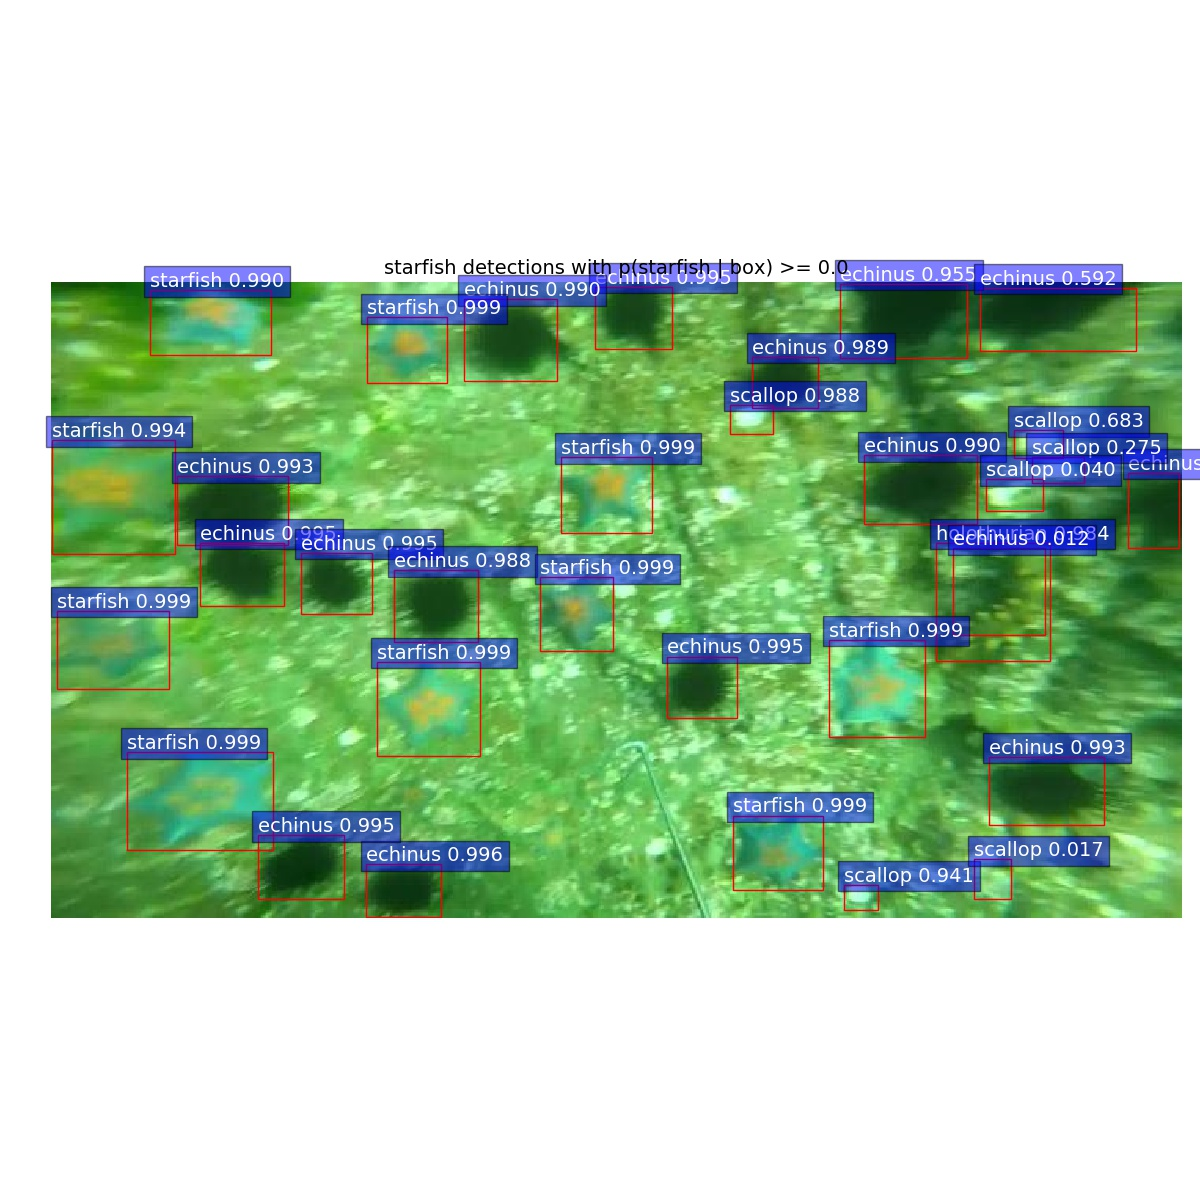
\includegraphics[width=7cm]{figures/6.jpg} 
		} 
		\subfigure[]{ 
			\label{p3b} %% label for second subfigure 
			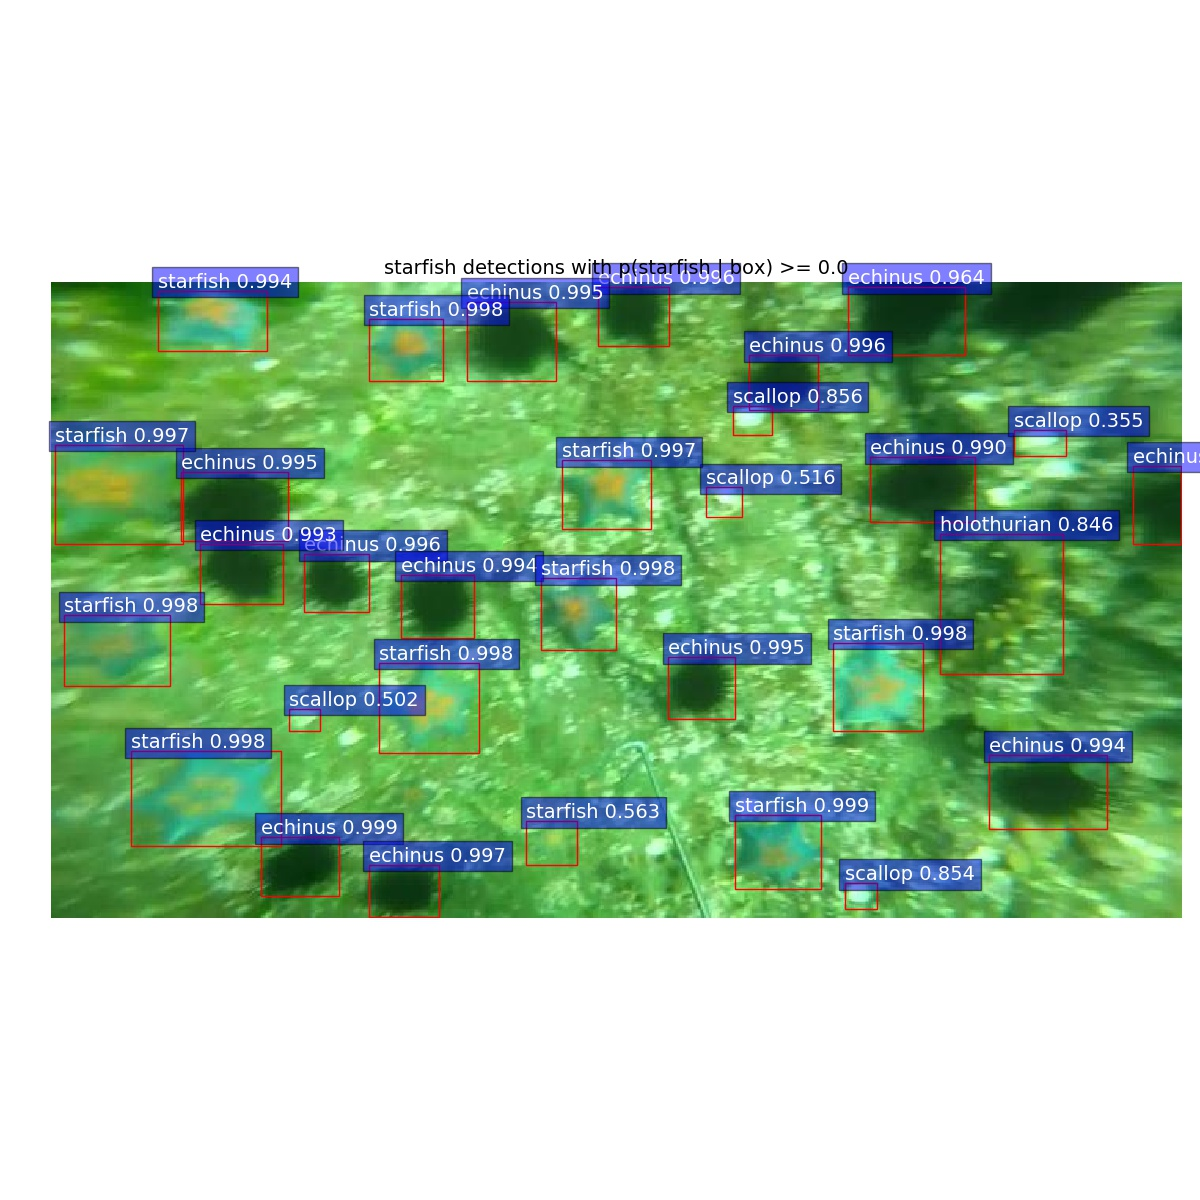
\includegraphics[width=7cm]{figures/7.jpg} 
		} 
		\subfigure[]{ 
			\label{p3c} %% label for second subfigure 
			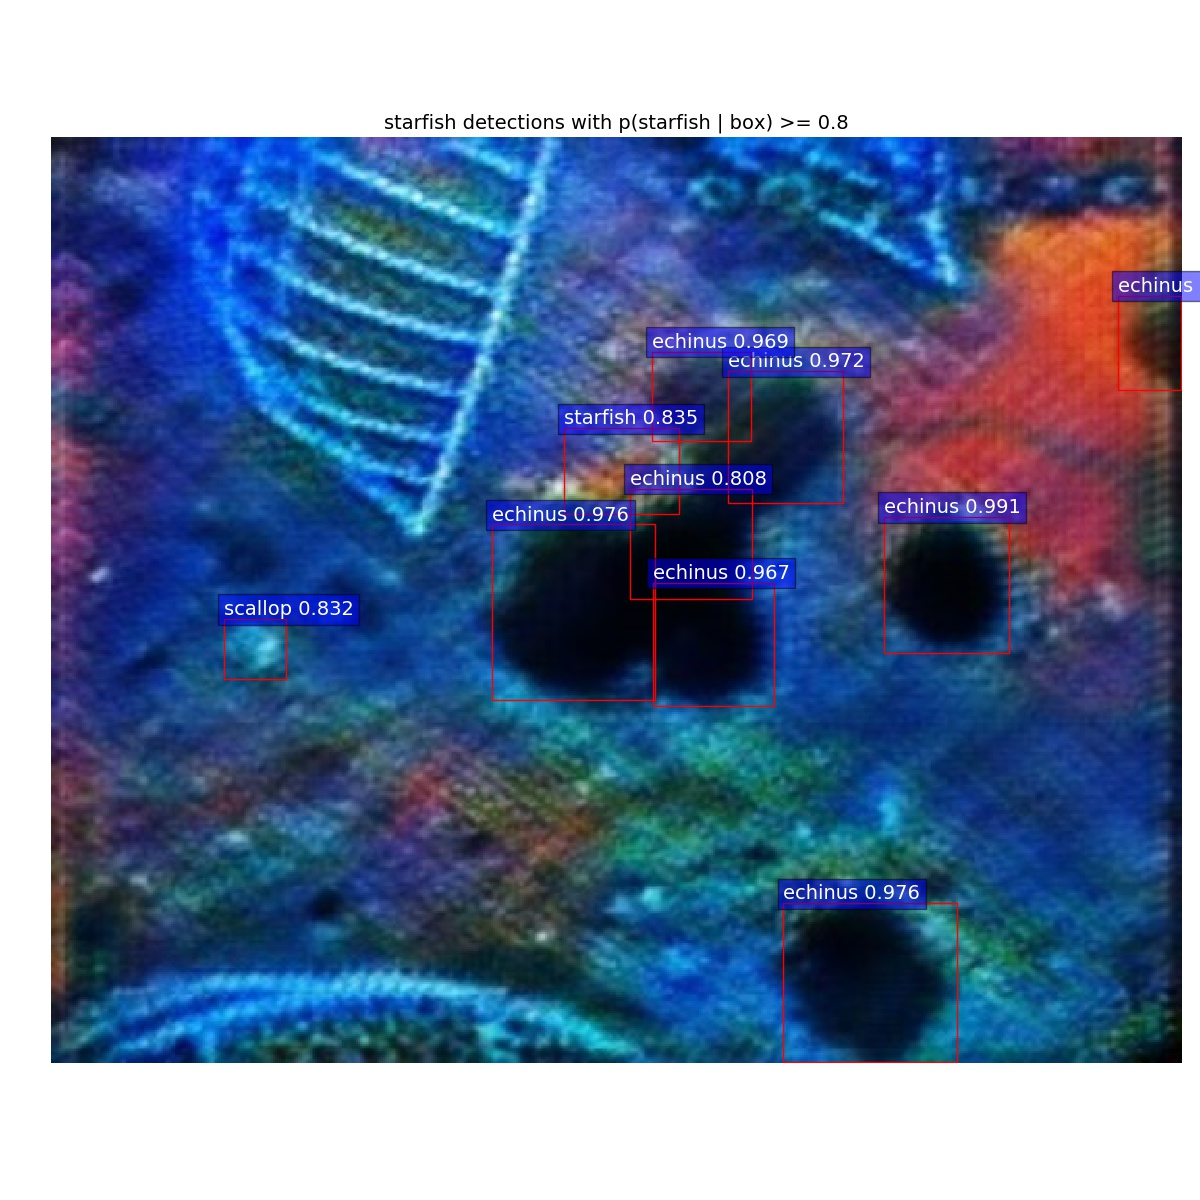
\includegraphics[width=7cm]{figures/8.jpg} 
		}
		\subfigure[]{ 
			\label{p3d} %% label for second subfigure 
			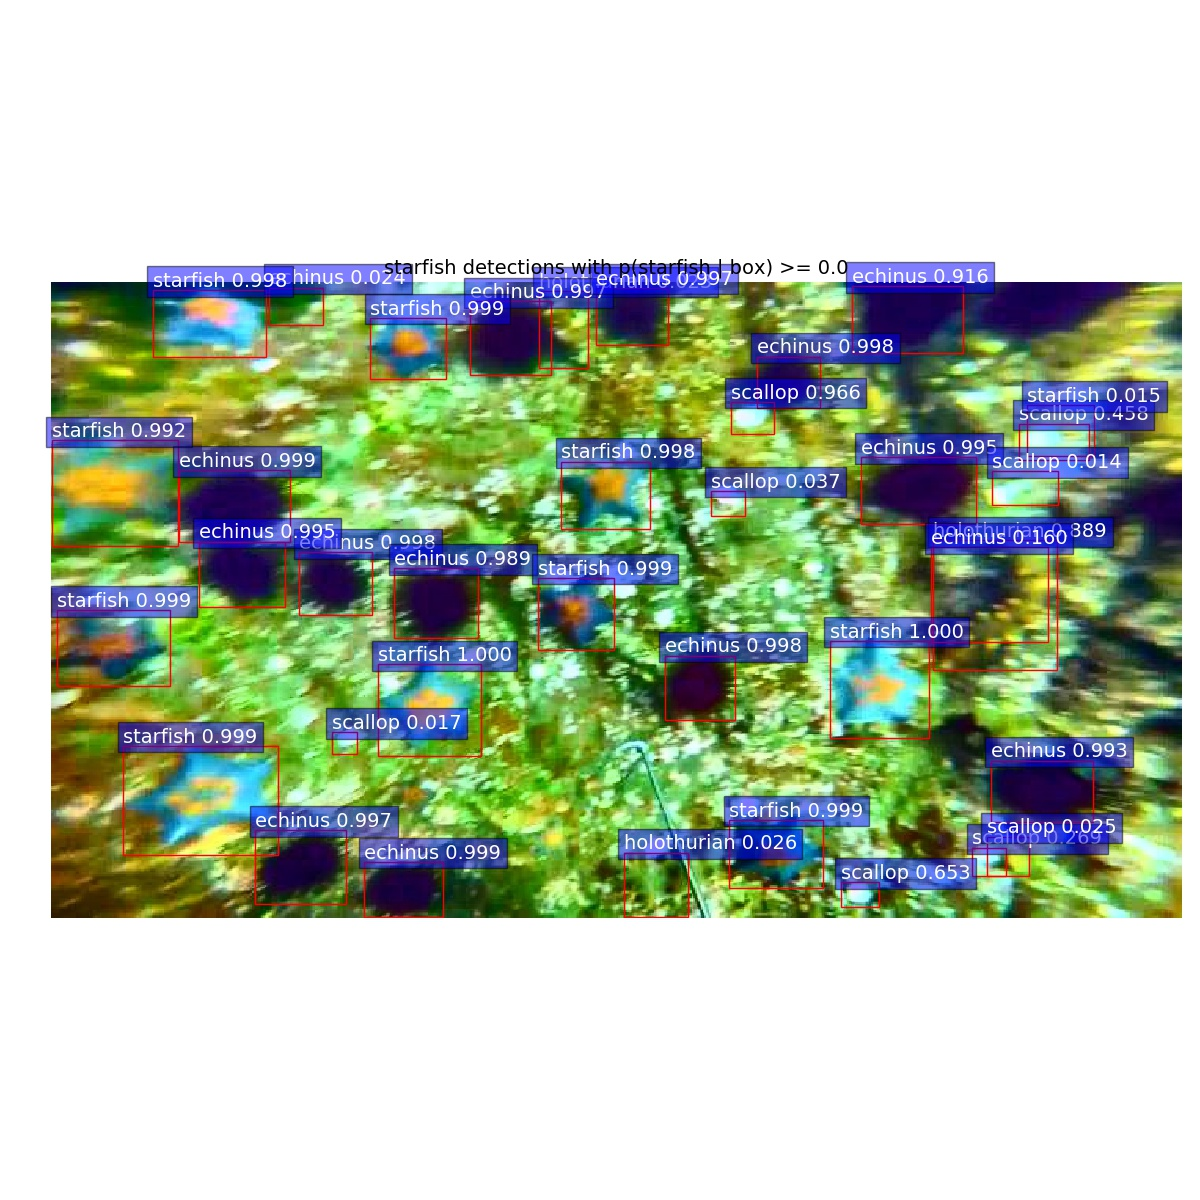
\includegraphics[width=7cm]{figures/9.jpg} 
		}
		\caption{Pictures with bounding boxes which are tested by different models.} 
		\label{p3} %% label for entire figure 
	\end{figure}
	
	\section{Progress in this week}
	
	When we are in URPC2018 site, I have trained offline and online models for competition. And we finish online and offline testing on site smoothly.
	\begin{description}
		\item[Step 1] Finish training an online contest model.
		\item[Step 2] Finish testing four offline models.
		\item[Step 3] Finish comparing mAP value of different methods and decide which threshold value to use.
		\item[Step 4] Finish online and offline testing on site smoothly.\label{t2}
	\end{description}
	
	\subsection{Contest Models Preparation}
	
	In order to prepare model weights for offline and online, I train several mdoels with cla2, cla6, hsv, dcp, dcp\_guided, dcp with clahe, cycle ssim, cycle ssim5 and so on. On this basis, I test them with some threshold from 0.8 to 0.001 and get results as shown in Fig.~\ref{p1}. Finally, when we are in game site, I choose threshold equal to 0.01 with original model weight.
	
	Except for what we need to see mAP value for evaluation, I try to write codes to output visualization results, for example, marking objects that are given to the game with Algorithm~\ref{g1}.
	
\lstset{language=python}
\begin{lstlisting}
def demo(sess, net, image_name):
"""Detect object classes in an image using pre-computed object proposals."""
	
all_name = image_name + '.jpg'
im_file = os.path.join(cfg.DATA_DIR, 'demo', all_name)
im = cv2.imread(im_file)
	
timer = Timer()
timer.tic()
scores, boxes = im_detect(sess, net, im)
timer.toc()
print('Detection took {:.3f}s for {:d} object proposals'.format(timer.total_time, boxes.shape[0]))
	
CONF_THRESH = 0.01
NMS_THRESH = 0.3
im = im[:, :, (2, 1, 0)]
fig,ax = plt.subplots(figsize=(12, 12))
ax.imshow(im, aspect='equal')
	
for cls_ind, cls in enumerate(CLASSES[1:]):
cls_ind += 1 # because we skipped background
cls_boxes = boxes[:, 4*cls_ind:4*(cls_ind + 1)]
cls_scores = scores[:, cls_ind]
dets = np.hstack((cls_boxes,
cls_scores[:, np.newaxis])).astype(np.float32)
keep = nms(dets, NMS_THRESH)
dets = dets[keep, :]
	
vis_detections(im, cls, dets,ax,thresh=CONF_THRESH)
plt.axis('off')
plt.tight_layout()
plt.draw()
	
if __name__ == '__main__':
cfg.TEST.HAS_RPN = True  # Use RPN for proposals
args = parse_args()
cfg.USE_GPU_NMS = False
	
demonet = args.demo_net
dataset = args.dataset
tfmodel = os.path.join('output', demonet, DATASETS[dataset][0], 'default',
NETS[demonet][0])
	
	
if not os.path.isfile(tfmodel + '.meta'):
raise IOError(('{:s} not found.\nDid you download the proper networks from '
'our server and place them properly?').format(tfmodel + '.meta'))
	
tfconfig = tf.ConfigProto(allow_soft_placement=True)
tfconfig.gpu_options.allow_growth=True
sess = tf.Session(config=tfconfig)
	
if demonet == 'vgg16':
net = vgg16()
elif demonet == 'res101':
net = resnetv1(num_layers=101)
else:
raise NotImplementedError
net.create_architecture("TEST",5,
tag='default', anchor_scales=[8, 16, 32])
saver = tf.train.Saver()
saver.restore(sess, tfmodel)
	
print('Loaded network {:s}'.format(tfmodel))
fr = open('/home/ai/Liuhongzhi/tf-faster-rcnn-contest-2018/data/VOCdevkit2007/test_list.txt', 'r')
for im_name in fr:
	
im_name = im_name.strip()
im_name = im_name.split(' ')
print('~~~~~~~~~~~~~~~~~~~~~~~~~~~~~~~~~~~')
print('mainDemo for data/demo/{}{}'.format(im_name[0], '.jpg'))
print('mainDemo for data/demo/{}{}'.format(im_name[1], '.jpg'))
demo(sess, net, im_name[0])
plt.savefig("testfigs/" + im_name[0] + '.jpg')
#plt.show()
\end{lstlisting}\label{g1}
	
	
	\subsection{2018URPC Competition Site}
	
	Our offline contest began at 1 o'clock in the afternoon on September 2nd. The result of submission as shown in Fig.~\ref{p2}. We test pictures with origin model first and result as Fig.~\ref{p2}\subref{p2a}. Then we quickly test with enhanced model as Fig.~\ref{p2}\subref{p2b}. Thirdly, we test with 17\&18 model Fig.~\ref{p2}\subref{p2c}. At last, we test with dcp model Fig.~\ref{p2}\subref{p2d}. Thanks to our partners, I can get enhanced pictures to test and get results in time.
	
	Furthermore, I can visualization of test results with bounding boxes in pictures as shown in Fig.~\ref{p3}. We test pictures with origin model first and result as Fig.~\ref{p3}\subref{p3a}. Then we quickly test with enhanced model as Fig.~\ref{p3}\subref{p3b}. Thirdly, we test with 17\&18 model Fig.~\ref{p3}\subref{p3c}. At last, we test with dcp model Fig.~\ref{p3}\subref{p3d}. Thanks to our partners, I can get enhanced pictures to test and get results in time.
		
	\section{Plan}
	
	\begin{tabular}{rl}
		\textbf{Objective:} & Finish thesis with senior students for CVPR2019.\\
		\textbf{Deadline:} & 2018.11.16
	\end{tabular}
	
	\begin{description}
		\item[\normalfont 2018.09.03---2018.09.09] Finish reading CVPR2018 paper about AttnGAN \cite{Tao18attngan}.
		\item[\normalfont 2018.09.10---2018.09.16] Finish recurrenting results of table from CVPR2018 paper.
	\end{description}
	
	% If you don't cite any references, please comment the following two lines
	\bibliographystyle{ieee}
	\bibliography{ref.bib}
	
\end{document}